\documentclass{article}

% Bullet preamble
\renewcommand{\labelitemi}{$\bullet$}
\renewcommand{\labelitemii}{$\diamond$}
\renewcommand{\labelitemiii}{$\circ$}

\newcommand{\mytab}{\hspace{0.3cm}}

% Math preamble
\usepackage{amsmath, amsthm, amsfonts, amssymb, amsfonts}
\usepackage{xfrac}
\numberwithin{equation}{section}

% Table preamble
\usepackage{multirow}

% Image preamble
\usepackage{graphicx}
\usepackage{float}   % for controlling float position

%%%%%%%%%%%%%%
\usepackage{tikz}
\usetikzlibrary{automata, positioning, arrows, calc, fit}

\tikzset{
    ->, % makes the edges directed
    >=stealth', % makes the arrow heads bold
    node distance=3cm, % specifies the minimum distance between two nodes. Change if necessary.
    state/.style={
            draw,
            rounded corners=3mm, % set the radius of the rounded corners
            thick,
            fill=gray!20,
            inner sep=0pt, % reduces the padding inside the node
            minimum width=1.5cm, % set the minimum width of the node
            minimum height=0.8cm, % set the minimum height of the node
        },
    %every state/.style={thick, fill=gray!20}, % sets the properties for each ’state’ node
    initial text=$START$, % sets the text that appears on the start arrow
    initial distance=1cm, % determines the distance of the start arrow
    initial where=above % tells where the start arrow should terminate
}
%%%%%%%%%%%%%%%


% Package for hiding links, click-able references
\usepackage[hidelinks]{hyperref}

% Margion specification
\usepackage[margin=1in,left=1in,includefoot]{geometry}
% Header, footer and page number
\usepackage{fancyhdr}
\pagestyle{fancy}
%clear header and footer
\fancyhead{}
\fancyfoot{}
% put page number on right side of footer
\fancyfoot[R]{\thepage}
% remove header and footer line
\renewcommand{\headrulewidth}{0pt}
\renewcommand{\footrulewidth}{0pt}

\begin{document}
% Include title page
\begin{titlepage}
	\begin{center}
		% include a line (slope){length}
		\line(1, 0){\textwidth}\\
		\vspace{2mm}
		\huge{\bfseries Group Project Report\\Group D}\\
		\vspace{2mm}
		\line(1, 0){\textwidth}\\
		\vspace{3cm}
	\end{center}

	\begin{table}[H]
		\centering
		\begin{tabular}{r l}
			\textsc{Course Title:} & Group Project\\
			\textsc{Course Code:} & EMARO-MSA-2001\\
			&\\
			\textsc{Group Members:} & Ahmed Yesuf Nurye\\
			& Taye Tsehaye Alamrew\\
			& Dilge Vurmaz\\
			& Mete Ogulcan Ozduygu\\
			&\\
			&\\
			\textsc{Instructor:} & Pawel Maciag\\
		\end{tabular}
	\end{table}
	\vspace{4cm}
	\begin{center}
		\textsc{June 2023.}
	\end{center}
\end{titlepage}

% Table of contents
\tableofcontents
% Remove page number on table of contents
\thispagestyle{empty}
% clear the rest of the page
\cleardoublepage

% Reset page numbering
% Start page number from 1 on the next page
\pagenumbering{arabic}
\setcounter{page}{1}

% List of figures
\listoffigures
\addcontentsline{toc}{section}{\numberline{}List of figures}
\cleardoublepage

% List of tables
\listoftables
\addcontentsline{toc}{section}{\numberline{}List of tables}
\cleardoublepage

% Include Project description
\section*{Project description}{\label{sec:task}}
\addcontentsline{toc}{section}{\numberline{}Project description}
The main goal of this project is to:
\begin{itemize}
    \item Model kinematics of serial 6R robot
    \item Develop a trajectory planning algorithm that solves a given task
    (pick and place)
    \item Test all computations in the simulation environment thoroughly
    \item Execute given task in hardware
\end{itemize}

% Include direct kinematics section
\section{Direct kinematics}\label{sec:direct}
\subsection{Kinematic structure of the robot}\label{subsec:kine_struct}
The manipulator is a 6 DoF anthropomorphic arm with spherical wrist. The structure is
shown in Figure \ref{fig:kine_struct}.
\begin{figure}[H]
    \centering
    \includegraphics[width=0.5\textwidth]{images/kine_struct}
    \caption{Kinematic structure of the robot}
    \label{fig:kine_struct}
\end{figure}

% DH parameter
\subsection{Denavit-Hartenberg parameters}\label{subsec:dh}
We used the modified DH convention to perform the axis assignment and the result is shown
in Figure \ref{fig:kine_struct}.
The summary of the axis assignment is given below.
\begin{enumerate}
    \item Assign the $z_i$ axis along the $i^{th}$ axis of rotation.
          % Z axis assignment
          \begin{itemize}
              \item $i=1: z_1$ pointing up along axis 1 on the plane of the page.
              \item $i=2: z_2$ pointing into the page along axis 2.
              \item $i=3: z_3$ pointing into the page along axis 3.
              \item $i=4: z_4$ pointing up along axis 4 on the plane of the page.
              \item $i=5: z_5$ pointing into the page along axis 5.
              \item $i=6: z_6$ pointing to the right along axis 6 on the plane of the page.
          \end{itemize}
          % X axis assignment
    \item Find the common perpendiculars between the $z_{i-1}$ and $z_i$ axes.
          if those axes intersect the common perpendicular is defined along $z_{i-1}\times z_i$
    \item Define the $x_i$ axes. The axis $x_{i-1}$ coincides with the common perpendicular between
          axes $z_{i-1}$ and $z_i$ and points from $z_{i-1}$ to $z_i$.
\end{enumerate}
The DH parameters are defined as follows:
\begin{itemize}
    \item $a_{i-1}$: The distance between axes $z_{i-1}$ and $z_i$ measured along $x_{i-1}$
    \item $\alpha_{i-1}$: The angle between axes $z_{i-1}$ and $z_i$ measured around $x_{i-1}$
    \item $d_i$: The distance between axes $x_{i-1}$ and $x_i$ measured along $z_i$
    \item $\theta_i$: The angle between axes $x_{i-1}$ and $x_i$ measured around $z_i$
\end{itemize}
% DH table
\begin{table}[H]
    \centering
    \caption{DH parameters}
    \label{tab:dh}
    \begin{tabular}{|c|c|c|c|c|}
        \hline
        ${i}$ & $\alpha_{i-1}$ & $a_{i-1}$ & $d_i$ & $\theta_i$ \\\hline
        1     & 0              & 0         & $d_1$ & $\theta_1$ \\\hline
        2     & $-\pi/2$       & 0         & 0     & $\theta_2$ \\\hline
        3     & 0              & $a_2$     & 0     & $\theta_3$ \\\hline
        4     & $-\pi/2$       & $a_3$     & $d_4$ & $\theta_4$ \\\hline
        5     & $\pi/2$        & 0         & 0     & $\theta_5$ \\\hline
        6     & $-\pi/2$       & 0         & $d_6$ & $\theta_6$ \\
        \hline
    \end{tabular}
\end{table}
\subsection*{DH parameters verification}
The DH parameters have been verified using Peter Corke MATLAB robotics toolbox. The plot of the
robot at home position is shown in Figure \ref{fig:home}.
\begin{figure}[H]
    \centering
    \includegraphics[width=0.5\textwidth]{images/dh_home}
    \caption{DH parameters verification}
    \label{fig:home}
\end{figure}

% Homogeneous transformation matrices
\subsection{Homogeneous transformation matrices}\label{subsec:hom_transf}
For the sake of simplicity, we define the following notations:
\begin{equation}\label{eq:simplicity}
    \begin{split}
        c_i&=cos(\theta_i)\\
        s_i&=sin(\theta_i)\\
        c_{ij}&=cos(\theta_i+\theta_j)\\
        s_{ij}&=sin(\theta_i+\theta_j)
    \end{split}
\end{equation}

% Insert dh frame assignmnet image
\begin{figure}[H]
    \centering
    \includegraphics[width=0.5\textwidth]{images/dh_frame}
    \caption{DH frame assignment}
    \label{fig:dh_frame}
\end{figure}

From the frame assignment shown in Figure \ref{fig:dh_frame},
the homogenous transformation matrix between frame $i$ and fram $i-1$ is given by:
\begin{equation} \label{eq:transf}
    {_i^{i-1}}T=Rot(x_{i-1},\alpha_{i-1})Trans(x_{i-1},a_{i-1})Rot(z_i,\theta_i)Trans(z_i,d_i)
\end{equation}

\begin{equation} \label{eq:hom_transf}
    {_i^{i-1}}T=\begin{bmatrix}
        c_i                  & -s_i                 & 0                 & a_{i-1}              \\
        s_i c_{\alpha_{i-1}} & c_i c_{\alpha_{i-1}} & -s_{\alpha_{i-1}} & -d_is_{\alpha_{i-1}} \\
        s_i s_{\alpha_{i-1}} & c_i s_{\alpha_{i-1}} & c_{\alpha_{i-1}}  & d_ic_{\alpha_{i-1}}  \\
        0                    & 0                    & 0                 & 1
    \end{bmatrix}
\end{equation}
Now, by substituting the DH parameters from Table \ref{tab:dh} into Equation \ref{eq:hom_transf},
let's solve the direct kinematics problem.

\begin{equation} \label{eq:hom_transf_prod}
    {_6^{0}}T=\prod_{i=1}^{6}{_i^{i-1}}T
\end{equation}

\begin{equation} \label{eq:T10}
    {_1^{0}}T=\begin{bmatrix}
        c_1 & -s_1 & 0 & 0   \\
        s_1 & c_1  & 0 & 0   \\
        0   & 0    & 1 & d_1 \\
        0   & 0    & 0 & 1
    \end{bmatrix}
\end{equation}

\begin{equation} \label{eq:T21}
    {_2^{1}}T=\begin{bmatrix}
        c_2  & -s_2 & 0 & 0 \\
        0    & 0    & 1 & 0 \\
        -s_2 & -c_2 & 0 & 0 \\
        0    & 0    & 0 & 1
    \end{bmatrix}
\end{equation}

\begin{equation} \label{eq:T20}
    {_2^{0}}T=\begin{bmatrix}
        c_1c_2 & -c_1s_2 & -s_1 & 0   \\
        c_2s_1 & -s_1s_2 & c_1  & 0   \\
        -s_2   & -c_2    & 0    & d_1 \\
        0      & 0       & 0    & 1
    \end{bmatrix}
\end{equation}

\begin{equation} \label{eq:T32}
    {_3^{2}}T=\begin{bmatrix}
        c_3 & -s_3 & 0 & a_2 \\
        s_3 & c_3  & 0 & 0   \\
        0   & 0    & 1 & 0   \\
        0   & 0    & 0 & 1
    \end{bmatrix}
\end{equation}

\begin{equation} \label{eq:T30}
    {_3^{0}}T=\begin{bmatrix}
        c_{23}c_1 & -s_{23}c_1 & -s_1 & a_2c_1c_2  \\
        c_{23}s_1 & -s_{23}s_1 & c_1  & a_2c_2s_1  \\
        -s_{23}   & -c_{23}    & 0    & d_1-a_2s_2 \\
        0         & 0          & 0    & 1
    \end{bmatrix}
\end{equation}

\begin{equation} \label{eq:T43}
    {_4^{3}}T=\begin{bmatrix}
        c_4  & -s_4 & 0 & a_3 \\
        0    & 0    & 1 & d_4 \\
        -s_4 & -c_4 & 0 & 0   \\
        0    & 0    & 0 & 1
    \end{bmatrix}
\end{equation}

\begin{equation} \label{eq:T40}
    {_4^{0}}T=\begin{bmatrix}
        s_1s_4+c_{23}c_1c_4 & c_4s_1-c_{23}c_1s_4  & -s_{23}c_1 & c_1\left(a_3c_{23}-d_4s_{23}+a_2c_2\right) \\
        c_{23}c_4s_1-c_1s_4 & -c_1c_4-c_{23}s_1s_4 & -s_{23}s_1 & s_1\left(a_3c_{23}-d_4s_{23}+a_2c_2\right) \\
        -s_{23}c_4          & s_{23}s_4            & -c_{23}    & d_1-d_4c_{23}-a_3s_{23}-a_2s_2             \\
        0                   & 0                    & 0          & 1
    \end{bmatrix}
\end{equation}

\begin{equation} \label{eq:T54}
    {_5^{4}}T=\begin{bmatrix}
        c_5 & -s_5 & 0  & 0 \\
        0   & 0    & -1 & 0 \\
        s_5 & c_5  & 0  & 0 \\
        0   & 0    & 0  & 1
    \end{bmatrix}
\end{equation}

\begin{equation} \label{eq:T50}
    {_5^{0}}T=\begin{bmatrix}
        % 1st row
        \begin{aligned}
             & c_5\left(s_1s_4 + c_{23}c_1c_4\right) \\
             & -s_{23}c_1s_5
        \end{aligned}  &
        \begin{aligned}
             & -s_5\left(s_1s_4 + c_{23}c_1c_4\right) \\
             & -s_{23}c_1c_5
        \end{aligned} & c_{23}c_1s_4 - c_4s_1    &
        c_1\left(a_3c_{23} - d_4s_{23} + a_2c_2\right)                                                                                                       \\\\
        % 2nd row
        \begin{aligned}
             & -c_5\left(c_1s_4 - c_{23}c_4s_1\right) \\
             & - s_{23}s_1s_5
        \end{aligned} &
        \begin{aligned}
             & s_5\left(c_1s_4 - c_{23}c_4s_1\right) \\
             & - s_{23}c_5s_1
        \end{aligned}  & c_1c_4 + c_{23}s_1s_4    & s_1(a_3c_{23} - d_4s_{23} + a_2c_2)                                                                      \\\\
        % 3rd row
        - c_{23}s_5 - s_{23}c_4c_5                   & s_{23}c_4s_5 - c_{23}c_5 & -s_{23}s_4                          & d_1 - d_4c_{23} - a_3s_{23} - a_2s_2 \\\\
        0                                            & 0                        & 0                                   & 1
    \end{bmatrix}
\end{equation}

\begin{equation} \label{eq:T65}
    {_6^{5}}T=\begin{bmatrix}
        c_6  & -s_6 & 0 & 0   \\
        0    & 0    & 1 & d_6 \\
        -s_6 & -c_6 & 0 & 0   \\
        0    & 0    & 0 & 1
    \end{bmatrix}
\end{equation}

% Direct kinematics
\begin{equation} \label{eq:T60}
    \setlength{\arraycolsep}{1pt}
    {_6^{0}}T=\begin{bmatrix}
        % 1st row
        \begin{aligned}
             & c_5c_6\left(s_1s_4 + c_{23}c_1c_4\right)\\
             & -s_{23}c_1c_6s_5 \\
             & +s_6\left(c_4s_1 - c_{23}c_1s_4\right)
        \end{aligned}   &
        \begin{aligned}
             & -c_5s_6\left(s_1s_4 + c_{23}c_1c_4\right) \\
             &+ s_{23}c_1s_5s_6 \\
             & +c_6\left(c_4s_1 - c_{23}c_1s_4\right)
        \end{aligned} &
        \begin{aligned}
             & -s_1s_4s_5 \\
             &- c_{23}c_1c_4s_5 \\
             & -s_{23}c_1c_5
        \end{aligned}                              &
        \begin{aligned}
             & c_1\left(a_3c_{23} - d_4s_{23} + a_2c_2\right)                        \\
             & -d_6s_5\left(s_1s_4 + c_{23}c_1c_4\right) \\
             &+ -d_6s_{23}c_1c_5
        \end{aligned}              \\\\
        % 2nd row
        \begin{aligned}
             & -c_5c_6\left(c_1s_4 - c_{23}c_4s_1\right) \\
             &- s_{23}c_6s_1s_5 \\
             & -s_6\left(c_1c_4 + c_{23}s_1s_4\right)
        \end{aligned} &
        \begin{aligned}
             & s_6c_5\left(c_1s_4 - c_{23}c_4s_1\right) \\
             &+ s_{23}s_1s_5s_6 \\
             & -c_6\left(c_1c_4 + c_{23}s_1s_4\right)
        \end{aligned}  &
        \begin{aligned}
             & c_1s_4s_5 \\
             &- c_{23}c_4s_1s_5 \\
             & -s_{23}c_5s_1
        \end{aligned}                               &
        \begin{aligned}
             & s_1\left(a_3c_{23} - d_4s_{23} + a_2c_2\right)                        \\
             & +d_6s_5\left(c_1s_4 - c_{23}c_4s_1\right) \\
             &- d_6s_{23}c_5s_1
        \end{aligned}              \\\\
        % 3rd row
        \begin{aligned}
             & -c_6c_{23}s_5 \\
             &- s_{23}c_4c_5c_6 \\
             & +s_{23}s_4s_6
        \end{aligned}                           &
        \begin{aligned}
             & c_{23}s_5s_6 \\
             &+ s_{23}c_4c_5s_6 \\
             & +s_{23}c_6s_4
        \end{aligned}                            &
        \begin{aligned}
             & s_{23}c_4s_5 \\
             & -c_{23}c_5
        \end{aligned}                                                        &
        \begin{aligned}
             & d_1 - d_4*c_{23} - a_3*s_{23} \\
             & - a_2s_2 -d_6c_{23}c_5 \\
             & + d_6s_{23}c_4s_5
        \end{aligned}                                          \\\\
        0                                                                         & 0 & 0 & 1
    \end{bmatrix}
\end{equation}


% Include inverse kinematics section
\section{Inverse Kinematics} \label{sec:inverse_kinematics}
Before solving the inverse kinematics problem, we need to find the singular confugurations of the manipulator
using the Jacobian matrix. The singular configurations are the configurations where the determinant of the Jacobian matrix is $0$

\subsection{Singular configurations} \label{subsec:singularity}
\subsubsection*{Geometric Jacobian}
All data necessary to compute the geometric Jacobian can be
extracted from the matrices derived while solving the Direct Kinematics
Problem.
\begin{equation} \label{eq:J}
    \mathcal{J}=\begin{bmatrix}
        \mathcal{J}_v \\
        \mathcal{J_\omega}
    \end{bmatrix}
\end{equation}

\begin{equation} \label{eq:Ti0}
    {_i^{0}}T=\begin{bmatrix}
        {_i^{0}}r_{11} & {_i^{0}}r_{12} & {_i^{0}}r_{13} & {_i^{0}}r_{i3} & {_i^{0}}P_x \\
        {_i^{0}}r_{21} & {_i^{0}}r_{22} & {_i^{0}}r_{23} & {_i^{0}}r_{i3} & {_i^{0}}P_y \\
        {_i^{0}}r_{31} & {_i^{0}}r_{32} & {_i^{0}}r_{33} & {_i^{0}}r_{i3} & {_i^{0}}P_z \\
        0              & 0              & 0              & 1              & 1
    \end{bmatrix}
\end{equation}
\begin{equation}
    \implies{_i^{0}}P=\begin{bmatrix}
        {_i^{0}}p_x \\
        {_i^{0}}p_y \\
        {_i^{0}}p_z
    \end{bmatrix}
    and \quad
    {_i^{0}}z=\begin{bmatrix}
        {_i^{0}}r_{13} \\
        {_i^{0}}r_{23} \\
        {_i^{0}}r_{33}
    \end{bmatrix}
\end{equation}
All joints of the manipulator are revolute. Threfore,
\begin{equation}
    \begin{split}
        \mathcal{J_\omega}&=\left[{_1^{0}}z \quad {_2^{0}} \quad z{_3^{0}} \quad z{_4^{0}} \quad z{_5^{0}} \quad z{_6^{0}}z\right]\\
        \mathcal{J}_v&=\left[{_1^{0}}z \times \left({_6^{0}}p-{_1^{0}}p\right) \quad {_2^{0}}z \times \left({_6^{0}}p-{_2^{0}}p\right) \quad
        {_3^{0}}z \times \left({_6^{0}}p-{_3^{0}}p\right) \quad {_4^{0}}z \times \left({_6^{0}}p-{_4^{0}}p\right) \quad
        {_5^{0}}z \times \left({_6^{0}}p-{_5^{0}}p\right) \quad {_6^{0}}z \times \left({_6^{0}}p-{_6^{0}}p\right)\right]
    \end{split}
\end{equation}
The determinant of the Jacobian matrix is computed using MATLAB's symbolic toolbox.
\begin{equation}
    \det\left(\mathcal{J}\right)=-a_2s_5\left(a_3s_3 + d_4c_3\right)\left(a_3c_{23}-d_4s_{23} + a_2c_2\right)
\end{equation}
Setting $\det\left(\mathcal{J}\right)=0$ results the following.
\begin{equation} \label{eq:singular_config}
    \begin{aligned}
         & a_2 = 0                            \\
         & s_5 = 0                            \\
         & a_3s_3 + d_4c_3 = 0                \\
         & a_3c_{23} - d_4s_{23} + a_2c_2 = 0
    \end{aligned}
\end{equation}
Now that we have established the singular configurations, we can proceed to solve the inverse kinematics problem.
Let the desired position and orientation of the end-effector be given by ${_6^{0}}T_d$ as:
\begin{equation} \label{eq:Td}
    {_6^{0}}T_d=\begin{bmatrix}
        r_{11} & r_{12} & r_{13} & q_x \\
        r_{21} & r_{22} & r_{23} & q_y \\
        r_{31} & r_{32} & r_{33} & q_z \\
        0      & 0      & 0      & 1
    \end{bmatrix}
\end{equation}
where $q_x$, $q_y$ and $q_z$ are the desired end-effector position. We will use Equation \ref{eq:inv}
to solve for the joint angles.
\begin{equation} \label{eq:inv}
    {_6^{0}}T={_6^{0}}T_d
\end{equation}
We can manipulate Equation \ref{eq:inv} to isolate each joint angle. To do that we need to find the inveses of some intermediate homogenous transformation matrices.
\begin{equation} \label{eq:TTinv}
    \begin{aligned}
        T      & =\begin{bmatrix}
                      n_x & o_x & a_x & q_x \\
                      n_y & o_y & a_y & q_y \\
                      n_z & o_z & a_z & q_z \\
                      0   & 0   & 0   & 1
                  \end{bmatrix}                   \\
        T^{-1} & =\begin{bmatrix}
                      n_x & n_y & n_z & -n_xq_x-n_yq_y-n_zq_z \\
                      o_x & o_y & o_z & -o_xq_x-o_yq_y-o_zq_z \\
                      a_x & a_y & a_z & -a_xq_x-a_yq_y-a_zq_z \\
                      0   & 0   & 0   & 1
                  \end{bmatrix}
    \end{aligned}
\end{equation}

% theta_1
\subsection{Solution for $\theta_1$}
Equation \ref{eq:T40}, \ref{eq:T10}, and \ref{eq:TTinv} are used to isolate $\theta_1$ as follows.
\begin{equation} \label{eq:t11}
    \begin{aligned}
        {_0^{1}}T{_4^{0}}T & ={_0^{1}}T{_6^{0}}T_d{_5^{6}}T{_4^{5}}T \\
        \implies{_4^{1}}T  & ={_4^{1}}T_d
    \end{aligned}
\end{equation}
The matrices are too big and are not written here. The sybolic analysis done using MATLAB is attached together with this report.
Equating ${_4^{1}}T_{2,4}={_4^{1}}T_{d2,4}$ results:
\begin{equation} \label{eq:t12}
    \begin{aligned}
         & q_yc_1 - q_xs_1 - d_6r_{23}c_1 + d_6r_{13}s_1=0               \\
         & c_1\left(q_y-d_6r_{23}\right) = s_1\left(q_x-d_6r_{13}\right) \\
         & \frac{s_1}{c_1}=\frac{q_y-d_6r_{23}}{q_x-d_6r_{13}}
    \end{aligned}
\end{equation}
Therefore,
\begin{equation} \label{eq:t13}
    \theta_1=\mathrm{atan2}\left(q_y-d_6r_{23},q_x-d_6r_{13}\right)
\end{equation}
To avoid sholder singularity, the following condition must be satiesfied.
\begin{equation} \label{eq:t1_singularity}
    q_y-d_6r_{23}\neq0 \land q_x-d_6r_{13}\neq0
\end{equation}

% theta_2
\subsection{Solution for $\theta_2$}
We will follow the same procedure as in the previous section.
Equation \ref{eq:t11} will be used to solve for $\theta_2$.
\begin{equation} \label{eq:t21}
    \begin{aligned}
        {_4^{1}}T_{1,4}                & ={_4^{1}}T_{d1,4}                              \\
        a_3c_{23} - d_4s_{23} + a_2c_2 & =q_xc_1 + q_ys_1 - d_6r_{13}c_1 - d_6r_{23}s_1
    \end{aligned}
\end{equation}
Let $E=q_xc_1 + q_ys_1 - d_6r_{13}c_1 - d_6r_{23}s_1$
\begin{equation} \label{eq:t22}
    a_3c_{23} - d_4s_{23} + a_2c_2=E
\end{equation}

\begin{equation} \label{eq:t23}
    \begin{aligned}
        {_4^{1}}T_{3,4}                 & ={_4^{1}}T_{d3,4}      \\
        -d_4c_{23} - a_3s_{23} - a_2s_2 & =q_z - d_1 - d_6r_{33}
    \end{aligned}
\end{equation}
Let $F=d_6r_{33}+d_1-q_z$
\begin{equation} \label{eq:t24}
    d_4c_{23} + a_3s_{23} + a_2s_2=F
\end{equation}
From Equation \ref{eq:t22} and \ref{eq:t24}, we can get the following new sets of equations.
\begin{equation} \label{eq:t25}
    \begin{aligned}
         & a_3c_{23} - d_4s_{23}=E-a_2c_2 \\
         & d_4c_{23} + a_3s_{23}=F-a_2s_2
    \end{aligned}
\end{equation}
Squaring both sides of Equation \ref{eq:t25} results:
\begin{equation}
    \begin{aligned}
         & a_3^2c_{23}^2 + d_4^2s_{23}^2-2a_3c_{23}d_4s_{23}=E^2+a_2^2c_2^2-2Ea_2c_2 \\
         & d_4^2c_{23}^2 + a_3^2s_{23}^2+2a_3c_{23}d_4s_{23}=F^2+a_2^2s_2^2-2Fa_2s_2
    \end{aligned}
\end{equation}
Adding Equation \ref{eq:t25} results:
\begin{equation} \label{eq:t26}
    \begin{aligned}
        a_3^2+d_4^2=E^2+F^2+a_2^2-2Ea_2c_2-2Fa_2s_2
    \end{aligned}
\end{equation}
Moving the unknowns to the left side of Equation \ref{eq:t26} results:
\begin{equation} \label{eq:t27}
    \begin{aligned}
        Ec_2+Fs_2=\frac{E^2+F^2+a_2^2-a_3^2-d_4^2}{2a_2}
    \end{aligned}
\end{equation}
Equation \ref{eq:t27} is obtained by assuming that $a_2\neq0$.
As can be seen from Equation \ref{eq:singular_config}, $a_2 = 0$ is one of
the singularity configurations. If $a_2=0$ then joint 2 and joint 3 will have the same
axis of rotation resulting in loss of one degree of freedom.\\
Let
\begin{equation} \label{eq:t28}
    K=\frac{E^2+F^2+a_2^2-a_3^2-d_4^2}{2a_2}
\end{equation}
Substituting Equation \ref{eq:t28} into Equation \ref{eq:t27} results:
\begin{equation} \label{eq:t29}
    Ec_2+Fs_2=K
\end{equation}
Equation \ref{eq:t29} can be solved by transforming it into polar form.
\begin{equation} \label{eq:t210}
    \begin{aligned}
         & r=\sqrt{E^2+F^2}                                            \\
         & \tan(\phi)=\frac{F}{E} \Rightarrow \phi=\mathrm{atan2}(F,E)
    \end{aligned}
\end{equation}
\begin{equation} \label{eq:t211}
    \begin{aligned}
        F & =rsin(\phi) \\
        E & =rcos(\phi)
    \end{aligned}
\end{equation}
Substituting Equation \ref{eq:t211} into Equation \ref{eq:t29} results:
\begin{equation} \label{eq:t212}
    \begin{aligned}
         & rcos(\phi)c_2+rsin(\phi)s_2=K \\
         & rcos(\phi-\theta_2)=K
    \end{aligned}
\end{equation}
Using Equation \ref{eq:t210} and Equation \ref{eq:t212} the value of $\theta_2$ is solved to be:
\begin{equation}
    \begin{aligned}
        \theta_2=\mathrm{atan2}(F,E) \pm \arccos\left(\frac{K}{sqrt{E^2+F^2}}\right)
    \end{aligned}
\end{equation}
Note, from Equation \ref{eq:singular_config} and Equation \ref{eq:t22} we can see that $E=0$ is
a singular confuguration and we need to take care of it on the programming.
% Theta 3
\subsection{Solution for $\theta_3$}
We can use Equation \ref{eq:T20}, Equation \ref{eq:T50}, Equation \ref{eq:Td}, and Equation \ref{eq:TTinv} are used to isolate $\theta_3$.
\begin{equation} \label{eq:t31}
    \begin{aligned}
        {_0^{2}}T{_5^{0}}T & ={_0^{2}}T{_6^{0}}T_d{_5^{6}}T \\
        {_5^{2}}T          & ={_5^{2}}T_d
    \end{aligned}
\end{equation}

\begin{equation} \label{eq:t32}
    \begin{aligned}
        {_5^{2}}T_{24}                                   & ={_5^{2}}T_{d24}                                        \\
        d_4c_3 + a_3s_3=d_1c_2 - q_zc_2 + d_6r_{33}c_2 - & q_xc_1s_2 - q_ys_1s_2 + d_6r_13c_1s_2 + d_6r_{23}s_1s_2
    \end{aligned}
\end{equation}
By rearranging Equation \ref{eq:t32} we can express it in terms of variable $E$ and $F$ that we have defined earier.
\begin{equation} \label{eq:t33}
    d_4c_3 + a_3s_3=c_2(d_6r_{33}+d_1-q_z)+s_2(c_1(d_6r_{13}-q_x) + s1(d_6r_{23}-q_y))
\end{equation}
Substituting $E$ and $F$ into Equation \ref{eq:t33} results:
\begin{equation} \label{eq:t34}
    d_4c_3 + a_3s_3=Fc_2-Es_2
\end{equation}
We can generate another equation using element $1,4$
\begin{equation} \label{eq:t35}
    \begin{aligned}
        {_5^{2}}T_{14}                                       & ={_5^{2}}T_{d14}                                            \\
        a_2 + a_3c_3 - d_4s_3=d_1s_2 - q_zs_2 + d_6r_{33}s_2 & + q_xc_1c_2 + q_yc_2s_1 - d_6r_{13}c_1c_2 - d_6r_{23}c_2s_1
    \end{aligned}
\end{equation}
By rearranging Equation \ref{eq:t35} we can express it in terms of variable $E$ and $F$ as well.
\begin{equation} \label{eq:t36}
    a_2 + a_3c_3 - d_4s_3=c_2(c_1(q_x-d_6r_{13}) + s_1(q_y-d_6r_{23})) + s_2(d_6r_{33}+d_1-q_z)
\end{equation}
Substituting $E$ and $F$ into Equation \ref{eq:t36} and moving $a_2$ to the right results:
\begin{equation} \label{eq:t37}
    a_3c_3 - d_4s_3=Ec_2+Fs_2-a_2
\end{equation}
Using the system of equation formed by Equation \ref{eq:t34} and Equation \ref{eq:t37} we can solve for $\theta_3$.
\begin{equation} \label{eq:t38}
    \begin{aligned}
        d_4c_3 + a_3s_3 & =Fc_2-Es_2     \\
        a_3c_3 - d_4s_3 & =Ec_2+Fs_2-a_2
    \end{aligned}
\end{equation}
Using variable change in $a_3$ and $d_4$ we can transform Equation \ref{eq:t38} into polar form and ulimately simplify
the system of equation.
\begin{equation} \label{eq:t39}
    \begin{aligned}
         & r=\sqrt{a_3^2+d_4^2}                                                 \\
         & \tan(\phi)=\frac{a_3}{d_4} \Rightarrow \phi=\mathrm{atan2}(a_3, d_4) \\
         & a_3=rsin(\phi)                                                       \\
         & d_4=rcos(\phi)
    \end{aligned}
\end{equation}
Substituting Equation \ref{eq:t39} into Equation \ref{eq:t38} results:
\begin{equation} \label{eq:t310}
    \begin{aligned}
        rc_\phi c_3 + rs_\phi s_3 & =Fc_2-Es_2     \\
        rs_\phi c_3 - rc_\phi s_3 & =Ec_2+Fs_2-a_2
    \end{aligned}
\end{equation}
Equation \ref{eq:t310} can be simplifies to:
\begin{equation} \label{eq:t311}
    \begin{aligned}
        rcos(\phi-\theta_3)   & =Fc_2-Es_2     \\
        rsin(\phi - \theta_3) & =Ec_2+Fs_2-a_2 \\
    \end{aligned}
\end{equation}
\begin{equation} \label{eq:t312}
    \tan\left(\phi - \theta_3\right)=\frac{Ec_2+Fs_2-a_2}{Fc_2-Es_2}
\end{equation}
Therefore,
\begin{equation} \label{eq:t313}
    \theta_3=\mathrm{atan2}(a_3, d_4) - \mathrm{atan2}(Ec_2+Fs_2-a_2, Fc_2-Es_2)
\end{equation}
One of the singularity confuguration term, $d_4c_3+a_3s_3$, appears while solving for $\theta_3$.
This fact is shown in Equation \ref{eq:t38}.
This singularity confuguration occures when the robot is fully stretched and it must as well be taken into
account when programming the robot.
% Theta 5
\subsection{Solution for $\theta_5$}
Equation \ref{eq:T30}, Equation \ref{eq:T50}, Equation \ref{eq:Td}, and Equation \ref{eq:TTinv} are used to isolate $\theta_5$.
\begin{equation} \label{eq:t51}
    \begin{aligned}
        {_0^{3}}T{_5^{0}}T & ={_0^{3}}T{_6^{0}}T_d{_5^{6}}T \\
        {_5^{3}}T          & ={_5^{3}}T_d
    \end{aligned}
\end{equation}

\begin{equation} \label{eq:t52}
    \begin{aligned}
        {_5^{3}}T_{22}                    & ={_5^{3}}T_{d22}                                                      \\
        c_5=r_{33}s_2s_3 - r_{33}c_2c_3 - & r_{13}c_1c_2s_3 - r_{13}c_1c_3s_2 - r_{23}c_2s_1s_3 - r_{23}c_3s_1s_2
    \end{aligned}
\end{equation}
Equation \ref{eq:t52} can be simplified to:
\begin{equation} \label{eq:t53}
    c_5=-s_{23}(r_{13}c_1+r_{23}s_1)-r_{33}c_{23}
\end{equation}
Let
\begin{equation} \label{eq:t54}
    A=r_{13}c_1+r_{23}s_1
\end{equation}
\begin{equation} \label{eq:t55}
    c_5=-r_{33}c_{23}-As_{23}
\end{equation}
Using the trigonometric identity $c_5^2+s_5^2=1$ we can solve for $s_5$ as follows:
\begin{equation} \label{eq:t56}
    s_5=\pm\sqrt{1-c_5^2}
\end{equation}
Therefore,
\begin{equation} \label{eq:t57}
    \begin{aligned}
        \theta_5 & =\mathrm{atan2}(s_5, c_5)                                                                           \\
        \theta_5 & =\pm\mathrm{atan2}\left(\sqrt{1-\left(-r_{33}c_{23}-As_{23}\right)^2}, -r_{33}c_{23}-As_{23}\right)
    \end{aligned}
\end{equation}

% Theta 4
\subsection{Solution for $\theta_4$}
Equation \ref{eq:t51} will be used to solve for $\theta_4$ as well.
\begin{equation} \label{eq:t41}
    \begin{aligned}
        {_5^{3}}T_{32} & ={_5^{3}}T_{d32}       \\
        s_4s_5         & =r_{23}c_1 - r_{13}s_1
    \end{aligned}
\end{equation}
Let $B=r_{23}c_1 - r_{13}s_1$
\begin{equation} \label{eq:t42}
    s_4s_5=B
\end{equation}
We can construct another Equation using element $1, 2$ of the same matrix as follows.
\begin{equation} \label{eq:t43}
    \begin{aligned}
        {_5^{3}}T_{12}                                        & ={_5^{3}}T_{d12}                                      \\
        -c_4s_5=r_{13}c_1c_2c_3 - r_{33}c_3s_2 - r_{33}c_2s_3 & + r_{23}c_2c_3s_1 - r_{13}c_1s_2s_3 - r_{23}s_1s_2s_3
    \end{aligned}
\end{equation}
Equation \ref{eq:t43} can be simplified to:
\begin{equation} \label{eq:t44}
    \begin{aligned}
        -c_4s_5=(r_{13}c_1+r_{23}s_1)c_{23}-r_{33}s_{23} \\
        \Rightarrow c_4s_5=r_{33}s_{23}-Ac_{23}
    \end{aligned}
\end{equation}
From Equation \ref{eq:t42} and Equation \ref{eq:t44} we can construct Equation \ref{eq:t45}.
\begin{equation} \label{eq:t45}
    \begin{aligned}
        s_4s_5 & =B                    \\
        c_4s_5 & =r_{33}s_{23}-Ac_{23}
    \end{aligned}
\end{equation}
Therefore, assuming that $s_5\neq0$, we can solve for $\theta_4$ as follows:
\begin{equation} \label{eq:t46}
    \theta_4=\mathrm{atan2}(B, r_{33}s_{23}-Ac_{23})
\end{equation}
Note that $s_5=0$ is one of the singularity configurations. We will solve for $\theta_4$ in this case later.
% Theta 6
\subsection{Solution for $\theta_6$}
We can isolate $\theta_6$ using Equation \ref{eq:T50}, Equation \ref{eq:T65}, Equation \ref{eq:Td}, and Equation \ref{eq:TTinv}.
\begin{equation} \label{eq:t61}
    \begin{aligned}
        {_6^{5}}T & ={_0^{5}}T{_6^{0}}T_d \\
        {_6^{5}}T & ={_6^{5}}T_d
    \end{aligned}
\end{equation}
\begin{equation} \label{eq:t62}
    \begin{split}
        {_6^{5}}T_{11}&={_6^{5}}T_{d11}\\
        c_6=r_{11}c_5s_1s_4 - r_{31}s_{23}c_4c_5 &- r_{11}s_{23}c_1s_5 - r_{21}s_{23}s_1s_5 - r_{21}c_1c_5s_4 \\
        &- r_{31}c_{23}s_5 + r_{21}c_{23}c_4c_5s_1 + r_{11}c_{23}c_1c_4c_5
    \end{split}
\end{equation}
Collecting like terms of Equation \ref{eq:t62} results:
\begin{equation} \label{eq:t63}
    \begin{aligned}
        c_6= & r_{11}\left(c_5s_1s_4+c_1(c_2(c_3c_4c_5-s_3s_5)-s_2(c_4c_5s_3+c_3s_5))\right)       \\
             & -r_{21}\left(c_4c_5s_1s_2s_3+c_1c_5s_4+c_3s_1s_2s_5+c_2s_1(s_3s_5-c_3c_4c_5)\right) \\
             & +r_{31}\left(s_3(s_2s_5-c_2c_4c_5)-c_3(c_4c_5s_2+c_2s_5)\right)
    \end{aligned}
\end{equation}
Using element $1, 2$ of the same matrix we can construct another equation as follows:
\begin{equation} \label{eq:t64}
    \begin{split}
        {_6^{5}}T_{12}&={_6^{5}}T_{d12}\\
        -s_6=r_{12}c_5s_1s_4 - r_{32}s_{23}c_4c_5 &- r_{12}s_{23}c_1s_5 - r_{22}s_{23}s_1s_5 - r_{22}c_1c_5s_4 \\
        &- r_{32}c_{23}s_5 + r_{22}c_{23}c_4c_5s_1 + r_{12}c_{23}c_1c_4c_5
    \end{split}
\end{equation}
Collecting like terms of Equation \ref{eq:t64} results:
\begin{equation} \label{eq:t65}
    \begin{aligned}
        -s_6=&r_{12}(c_5s_1s_4+c_1(c_2(c_3c_4c_5-s_3s_5)-s_2(c_4c_5s_3+c_3s_5)))\\
        &-r_{22}(c_4c_5s_1s_2s_3 + c_1c_5s_4 + c_3s_1s_2s_5 + c_2s_1 (s_3s_5 - c_3c_4c_5))\\
        &+r_32(s_3(s_2s_5-c_2c_4c_5)-c_3(c_4c_5s_2+c_2s_5))
    \end{aligned}
\end{equation}
Therefore, using Equation \ref{eq:t63} and Equation \ref{eq:t65} $\theta_6$ can be solved as follows:
\begin{equation} \label{eq:t66}
    \theta_6=\mathrm{atan2}(s_6,c_6)
\end{equation}
% Theta 6 and 4 when s5=0
Now let's solve for $\theta_4$ and $\theta_6$ when $s_5=0$, i.e., when there is a wrist singularity.
This condition results when $z_4$ and $z_6$ coincides. Resulting in cancellation of motion of joint 4 and joint 6.
Equation \ref{eq:T10}, Equation \ref{eq:T60}, Equation \ref{eq:Td}, and Equation \ref{eq:TTinv} are used to isolate $\theta_4$ and $\theta_6$.
\begin{equation} \label{eq:t641}
    \begin{aligned}
        {_0^{1}}T{_6^{0}}T & ={_0^{1}}T{_6^{0}}T_d \\
        {_6^{1}}T & ={_6^{1}}T_d
    \end{aligned}
\end{equation}
\begin{equation} \label{eq:t642}
    \begin{aligned}
        {_6^{1}}T_{21} & ={_6^{1}}T_{d21}\\
        -c_4s_6 - c_5c_6s_4 &= r_{21}c_1 - r_{11}s_1
    \end{aligned}
\end{equation}
Using element $2, 2$ of the same matrix we can construct another equation as follows:
\begin{equation} \label{eq:t643}
    \begin{aligned}
        {_6^{1}}T_{22} & ={_6^{1}}T_{d22}\\
        c_5s_4s_6 - c_4c_6 &= r_{22}c_1 - r_{12}s_1
    \end{aligned}
\end{equation}
Simplifying Equation \ref{eq:t642} and Equation \ref{eq:t643} results Equation \ref{eq:t644}.
\begin{equation} \label{eq:t644}
    \begin{aligned}
        -\sin(\theta_6\pm\theta_4) &= r_{21}c_1 - r_{11}s_1 \\
        -\cos(\theta_6\pm\theta_4) &= r_{22}c_1 - r_{12}s_1
    \end{aligned}
\end{equation}
In wrist singularity confuguration $\theta_4$ and $\theta_6$ produces a motion that will effectively cancel each other. 
Therefore, it is logical to fix the value of one of those angles to its previous value ans solve for the other.\\
By fixing $\theta_4$ to its previous value, $\theta_{4prev}$, we can solve for $\theta_6$ as follows:
\begin{equation} \label{eq:t645}
    \begin{aligned}
        \theta_4&=\theta_{4prev}\\
        \theta_6&=\mathrm{atan2}\left(-(r_{21}c_1 - r_{11}s_1), -(r_{22}c_1 - r_{12}s_1)\right)\mp\theta_{4prev}
    \end{aligned}
\end{equation}

% Include kinematics test section
\section{kinematics tests}
Both forward and inverse kinematics are tested against Peter Corke's Robotics Toolbox MATLAB, use script $test\_kinematics$. \\
\textbf{\textcolor{red}{IMPORTANT:}} for the test it is required that \href[]{https://petercorke.com/toolboxes/robotics-toolbox/}{\textcolor{blue}{Peter Corke's Robotics Toolbox}} is installed. 
This is because we used the result from this toolbox as the ground truth.\\ 

Usage:\\
\texttt{>> test\_kinematics}\\
\subsection{Direct kinematics test}
Ten randomly generated joint angles are used to test the direct kinematics. We have used tolerance of $1e_-6$, 
and for this tolerance all the tests are passed. The test result is shown in Figure \ref{fig:direct_kinematics_test}.
\begin{figure}[H]
    \centering
    \includegraphics[width=0.4\textwidth]{images/direct_kinematics_test.png}
    \caption{Direct kinematics test}
    \label{fig:direct_kinematics_test}
\end{figure}

\subsection{Inverse kinematics test}
Similarly, ten homogeneous transformation matrices generated from 10 randomly generated joint angles 
are used to test the inverse kinematics. 
After calculating the inverse kinematics we recalculate the homogeneous transformation matrix and compare it with 
the original homogeneous transformation matrix. The same tolerance of $1e_-6$ is used and all the tests are passed.
The test result is shown in Figure \ref{fig:inverse_kinematics_test}.
\begin{figure}[H]
    \centering
    \includegraphics[width=0.4\textwidth]{images/inverse_kinematics_test.png}
    \caption{Inverse kinematics test}
    \label{fig:inverse_kinematics_test}
\end{figure}
% Include trajectory planning section
\section{Trajectory planning} \label{sec:trajectory_planning}
\textbf{\textcolor{red}{IMPORTANT:}} to simulate the trajectory it is required that \href[]{https://petercorke.com/toolboxes/robotics-toolbox/}{\textcolor{blue}{Peter Corke's Robotics Toolbox}} is installed.\\

Usage:\\
\texttt{>> test\_trajectory('j', true)}\\
\texttt{>> test\_trajectory('t', true)}\\

\textbf{Problem:} to find a trajectory connecting initial and final points.\\
There are different methods for trajectory jeneration. Some of them are:
\begin{itemize}
    \item LSPB
    \item Polynomial (Qubic, Quintic)
\end{itemize}
In this section we will perform the trajectory planning of simple pick and place task using LSPB.
We used both joint space and task space trajectory planning as shown in Figure \ref{fig:trajectory_planning} below.
\begin{figure}[H]
    \centering
    \begin{tikzpicture}
        \coordinate (A) at (0,0,0);
        \coordinate (B) at (2,0,0);
        \coordinate (C) at (2,2,0);
        \coordinate (D) at (0,2,0);
        \coordinate (E) at (0,0,2);
        \coordinate (F) at (2,0,2);
        \coordinate (G) at (2,2,2);
        \coordinate (H) at (0,2,2);

        \draw (A) -- (B) -- (C) -- (D) -- cycle;
        \draw (E) -- (F) -- (G) -- (H) -- cycle;
        \draw (A) -- (E);
        \draw (B) -- (F);
        \draw (C) -- (G);
        \draw (D) -- (H);

        \coordinate (I) at (5,0,0);
        \coordinate (J) at (7,0,0);
        \coordinate (K) at (7,2,0);
        \coordinate (L) at (5,2,0);
        \coordinate (M) at (5,0,2);
        \coordinate (N) at (7,0,2);
        \coordinate (O) at (7,2,2);
        \coordinate (P) at (5,2,2);

        \draw (I) -- (J) -- (K) -- (L) -- cycle;
        \draw (M) -- (N) -- (O) -- (P) -- cycle;
        \draw (I) -- (M);
        \draw (J) -- (N);
        \draw (K) -- (O);
        \draw (L) -- (P);

        \node at (0.85,2.8,0) {$*$};
        \node at (5.85,2.8,0) {$*$};
        \node at (0.85,1,0) {$*$};
        \node at (5.85,1,0) {$*$};
        % home
        \node at (-2,7,0) {$*$};

        \draw[-,red] (0.85,2.8,0) -- (0.85,1,0);
        \draw[-,red] (5.85,1,0) -- (5.85,2.8,0);

        \draw[-,blue] (-2,7) to[out=0, in=90] (0.85,2.8, 0);
        \draw[-,blue] (-2,7) to[out=0, in=90] (5.85,2.8, 0);
        \draw[-,blue] (0.85,2.8,0) to[out=90, in=90] (5.85,2.8, 0);

        % Legend
        \node[left] at (-2.7,7) {Home};
        \draw[-,blue] (8,7) -- (9,7);
        \draw[-,red] (8,6.5) -- (9,6.5);

        \node[right] at (9,7) {Joint space};
        \node[right] at (9,6.5) {Task space};

    \end{tikzpicture}
    \caption{Trajectory planning}
    \label{fig:trajectory_planning}
\end{figure}
The task definition can easly be seen from Figure \ref{fig:trajectory_planning}. 
In the next sub-sections we are going to see the implementation of task space and joint space trajectory planning.

\subsection{Joint space trajectory planning using LSPB}
What is LSPB?\\
In short, Linear Segments with Parabolic Blends trajectory, is a symmetric trajectory with
trapezoidal shape of velocity profile, with constant velocity in central part of the path.
\begin{itemize}
    \item This type of trajectory is appropriate when a constant velocity is
             desired along a portion of the path.
    \item The LSPB trajectory is such that the velocity is initially ramped up
             to its desired value and then ramped down when it approaches the
              goal position.
    \item To achieve this we specify the desired trajectory in three parts.
    \item For $t\in\left[t_0 \quad t_b\right]$ and $t\in\left[t_f-t_b \quad t_f\right]$ the trajectory is described by a quadratic polynomial.
    \item For $t\in\left[t_b \quad t_f - t_b\right]$ a constant velocity, $v$, is taken.
    \item The blend time $t_b$ is chosen such that the position curve is symmetric.
\end{itemize}
The LSPB trajectory is defined by the following equation, assuming $t_0=0$:
\begin{equation} \label{eq:lspb}
    \begin{cases}
        \theta(t) = \theta_0 + \frac{\alpha}{2} t^2 & 0 \leq t \leq t_b \\
        \theta(t) = \frac{\theta_0+\theta_f-vt_f}{2} + vt_f & t_b < t \leq t_f - t_b \\
        \theta(t) = \theta_f - \frac{\alpha t_f^2}{2} + \alpha t_f - \frac{\alpha}{2}t^2 & t_f - t_b < t \leq t_f
    \end{cases}
\end{equation}

\subsubsection{Constraints of LSPB}
While driving Equation \ref{eq:lspb} it is assumed that $0 \le t_b \le \frac{t_f}{2}$, Other wise the trajectory can't be achieved. 
From this condition we can derive the following constraints:
\begin{equation} \label{eq:lspb_constraints}
    \begin{aligned}
        \frac{q_f-q_0}{v} < t_f \le \frac{2(q_f-q_0)}{v} \\
        \implies \frac{q_f-q_0}{t_f} < v \le \frac{2(q_f-q_0)}{t_f}
    \end{aligned}
\end{equation}
If $t_b = \frac{t_f}{2}$ then the trajectory reduces to mimimum time trajectory (Bang-Bang trajectory).
We have used equation \ref{eq:lspb} to define the trajectory in joint space and the result for sample trajectory between the following initial 
and final joint angles is shown in Figure \ref{fig:lspb_single} and \ref{fig:lspb_trajectory}.

For a single joint: $q_0 = 0\, and \, q_f = \pi$
\begin{figure}[H]
    \centering
    \includegraphics[width=0.5\textwidth]{images/lspb_single_joint.png}
    \caption{LSPB trajectory for a single joint}
    \label{fig:lspb_single}
\end{figure}
For all the joints:
\begin{equation*}
    \begin{aligned}
        \theta_0 &= \begin{bmatrix}
            0 & 0 & 0 & 0 & 0 & 0
        \end{bmatrix}\\
        \theta_f &= \begin{bmatrix}
            \pi & \pi/2 & \pi/4 & \pi/6 & \pi/8 & \pi/10
        \end{bmatrix}
    \end{aligned}
\end{equation*}

\begin{figure}[H]
    \centering
    \includegraphics[width=0.5\textwidth]{images/lspb_trajectory.png}
    \caption{Synchronized LSPB trajectory}
    \label{fig:lspb_trajectory}
\end{figure}
For synchronizing the trajectories we have used the maximum $t_f$ of all the joints. 
This computation of time is implemented in the function $get\_time$.

\subsection{Task space trajectory planning}
For the task space trajectory planning we have followed the following steps:
\begin{itemize}
    \item Express the end-effector pose in terms of roll, pitch and yaw angles.
    \item Use linear interpolation to compute the trajectory for each of the roll, pitch and yaw angles 
          as well as the $X, Y, Z$ coordinates of the end effector (position).
    \item Convert each roll, pitch and yaw angles back to the rotation matrix.
    \item Generate the homogeneous transformation matrix using the rotation matrix and the position.
    \item Perform inverse kinematics to compute the joint angles for each of the homogeneous transformation matrix.
\end{itemize}
Note, if we don't generate enough points in the interpolation we can use LSPB to get more joint angles between each 
consequetive points.
The end-effector pose for straight line task space trajectory is shown in Figure \ref{fig:task_space_trajectory}.
\begin{figure}[H]
    \centering
    \includegraphics[width=0.6\textwidth, height=0.4\textheight]{images/task_space_trajectory.png}
    \caption{Task space Vs. Joint space trajectory, end-effector pose for triangular profile.}
    \label{fig:task_space_trajectory}
\end{figure}
Finally the pick and place task (contains both joint and task space trajectories) trajectory end-effector pose is shown in Figure \ref{fig:pick_and_place}.
\begin{figure}[H]
    \centering
    \includegraphics[width=0.5\textwidth]{images/pick_and_place_trajectory.png}
    \caption{Pick and place task}
    \label{fig:pick_and_place}
\end{figure}


% Include hardware section
\section{Hardware Implementation} \label{sec:hardware}
This section presents the step by step implementation of simple pick and place task in the real robot.

Usage:\\
\texttt{>> test\_pick\_and\_place}\\
\subsection{Hardware Setup} \label{subsec:hardware_setup}
At this stage we adjust the manipulator to the desired home position and recorded the joint angles corresponding to this home pose using Dynamixel wizard.
We also recorded the maximum and minimum joint angles for each motor using Dynamixel wizard.
The range of motion and velocity for each motor is shown in Table \ref{tab:range_of_motion_velocity}.
\begin{table}[h]
        \centering
        \caption{Range of motion and velocity for each motor}
        \label{tab:range_of_motion_velocity}
        \begin{tabular}{|c||c|l|}
                \hline
                \textbf{Motor Type} & \textbf{Range of Motion}     & \textbf{Velocity}               \\ \hline \hline
                Ax                  & $[0 - 1023] \to [0-300^0]  $ & $[0 - 1023]\to  [0-114rpm]$     \\ \hline
                Mx                  & $[0 - 4094] \to [0-360^0] $  & $ [0 - 1023] \to [0-116.62rpm]$ \\ \hline
        \end{tabular}
\end{table}

\subsection{Brief Description of the Code} \label{subsec:brief_description_code}
The functions used in the hardware implementation are listed below,
\begin{itemize}
        \item  $joint2motor$: converts joint angles from radian to manipulator units.
        \item  $traj\_pos\_joint2motor$: converts matrix of joint angles from radian to manipulator units by calling $joint2motor$ in a loop.
        \item  $vel\_rpm2dxl$: converts joint velocity from $rpm$ to manipulator units.
        \item  $traj\_vel\_joint2motor$: converts matrix of joint velocities from $rpm$ to manipulator units, by calling $vel\_rpm2dxl$ in a loop.
        \item  $open\_port$: establish communication by opening the port and setting the baud rate, specify the port from devide manager here.
        \item  $write\_data$: sends joint angles and velocities to all the motors simultaneously.
        \item  $sync\_send$: sends matrix of joint angles and velocities by calling $write\_data$ in a loop.
        \item  $gripper$: Opens and closes the gripper as required.
        \item  $close\_port$: for terminating session by closing the port.
        \item  $enable\_torque$: enables the torque of the manipulator motors, and also used to see if all the motors are working properly.
        \item  $disable\_torque$: disables the torque of the manipulator motors.
\end{itemize}
The script $test\_pick\_and\_place$ uses all the above functions to perform the pick and place task.

\cleardoublepage
\subsection{Pick and place task graph (Basic Algorithm)} \label{subsec:pick_and_place_task}
The task execution process is sequential and straightforward and is shown in Figure \ref{fig:fsm}.
%%%%%%%%%%%%%%%%%%%%%%%%%%%%%%%%%%%%%%%%%%%%%%%%%%%%
\begin{figure}[H] % ’ht’ tells LaTeX to place the figure ’here’ or at the top of the page
        \centering % centers the figure
        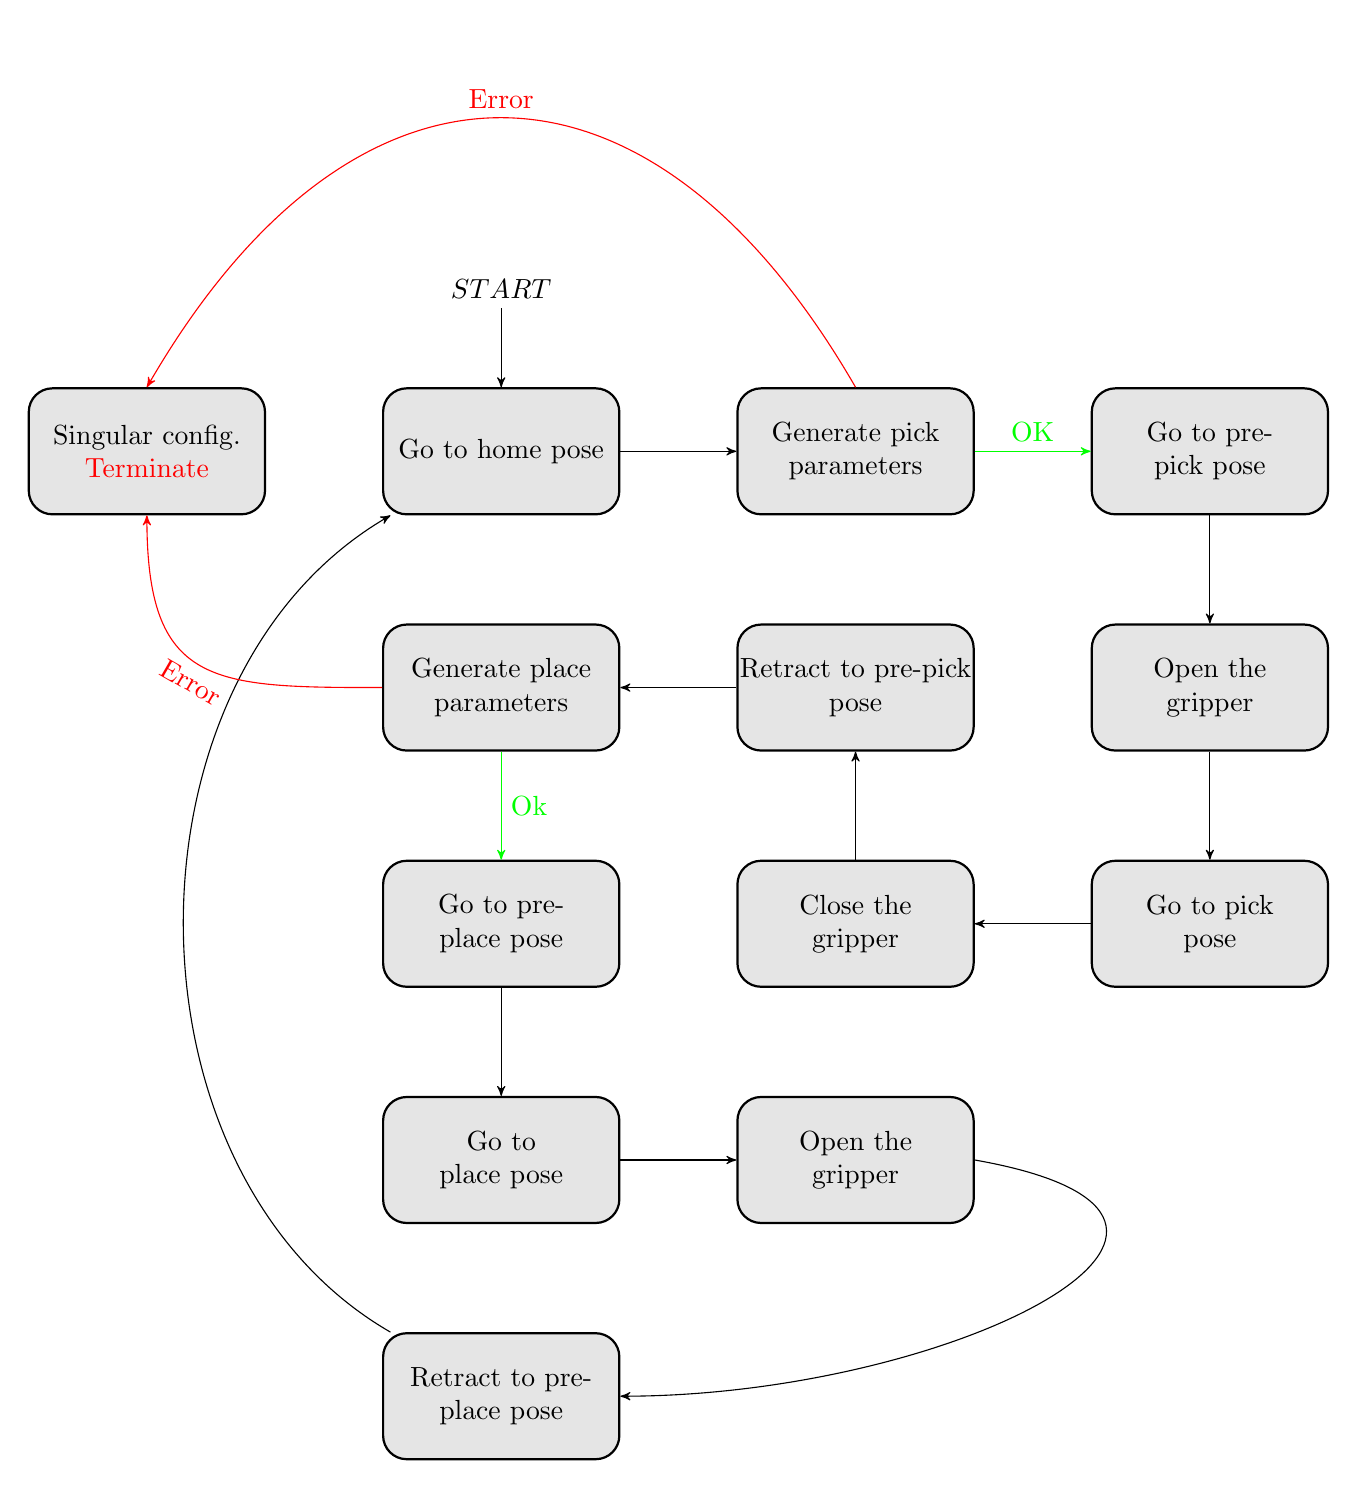
\begin{tikzpicture}
                % nodes
                \node[state, initial, minimum height=1.6cm, text width=3cm, align=center] (s1) {Go to home pose};
                \node[state, right of=s1, minimum height=1.6cm, xshift=1.5cm, text width=3cm, align=center] (s2) {Generate pick\\parameters};
                \node[state, right of=s2, minimum height=1.6cm, xshift=1.5cm, text width=3cm, align=center] (s3) {Go to pre-\\pick pose};
                \node[state, below of=s3, minimum height=1.6cm, text width=3cm, align=center] (s4) {Open the \\gripper};
                \node[state, below of=s4, minimum height=1.6cm,  text width=3cm, align=center] (s5) {Go to pick \\pose};
                \node[state, left of=s5, minimum height=1.6cm, xshift=-1.5cm, text width=3cm, align=center] (s6) {Close the \\gripper};
                \node[state, above of=s6, minimum height=1.6cm, text width=3cm, align=center] (s7) {Retract to pre-pick \\pose};
                \node[state, left of=s7, minimum height=1.6cm, xshift=-1.5cm, text width=3cm, align=center] (s8) {Generate place\\parameters};
                \node[state, below of=s8, minimum height=1.6cm, text width=3cm, align=center] (s9) {Go to pre-\\place pose};
                \node[state, below of=s9, minimum height=1.6cm, text width=3cm, align=center] (s10) {Go to \\place pose};
                \node[state, right of=s10, minimum height=1.6cm, xshift=1.5cm, text width=3cm, align=center] (s11) {Open the \\gripper};
                \node[state, below of=s10, minimum height=1.6cm, text width=3cm, align=center] (s12) {Retract to pre-\\place pose};

                \node[state, left of=s1, minimum height=1.6cm, xshift=-1.5cm,  text width=3cm, align=center] (e1) {Singular config. \\\textcolor{red}{Terminate}};


                % edges
                \draw[->] (s1) edge node[above] {} (s2);
                \draw[->, green] (s2) edge node[above] {OK} (s3);
                \draw[->] (s3) edge node[right] {} (s4);
                \draw[->] (s4) edge node[right] {} (s5);
                \draw[->] (s5) edge node[above] {} (s6);
                \draw[->] (s6) edge node[right] {} (s7);
                \draw[->] (s7) edge node[above] {} (s8);
                \draw[->, green] (s8) edge node[right] {Ok} (s9);
                \draw[->] (s9) edge node[right] {} (s10);
                \draw[->] (s10) edge node[right] {} (s11);
                \draw[->] (s11.east) to[out=-10, in=0, looseness=2] (s12.east);
                \draw[->] (s12) edge[bend left=60] node[above] {} (s1);

                \draw[->, red] (s2.north) to[out=120, in=60, looseness=1.5] node[above, sloped] {Error} (e1.north);
                \draw[->, red] (s8.west) to[out=180, in=-90, looseness=1.5] node[below, sloped] {Error} (e1.south);

        \end{tikzpicture}
        \caption{Task graph}
        \label{fig:fsm}
\end{figure}
%%%%%%%%%%%%%%%%%%%%%%%%%%%%%%%%%%%%%%%%%%%%%%%%%%%
Please note that, an  \textcolor{red}{error} is generated in the $inv\_kine$ function if a pose that results in singular confuguration is provided.\\
Please also note that the first initialization step before performing any task is to open the port, set baud rate, and enable torque.\\
The last steps are to disable the torque and close the port.\\\\
Description of the task graph:\\
\begin{enumerate}
        \item  Go to home pose: Initially the manipulator could be at any pose. Therefore, using the home pose joint angles recorded previously, we should go to the home pose first.
        \item  Generate pick parameters: Here we generate the trajectory to got to the pre-pick and pick poses. While performing the inverse kinematics we could encounter an error if singular configuration is provided.
        \item  Go to pre-pick pose: Done by sending the trajectory that connects home pose and pre-pick pose.
        \item  Open the gripper.
        \item  Go to pick pose.
        \item  Close the gripper.
        \item  Retract to pre-pick pose.
        \item  Generate place parameters: done in the same way as pick parameters are generated.
        \item  Go to pre-place pose: done in the same way as pre-pick pose is reached.
        \item  Go to place pose.
        \item  Open the gripper.
        \item  Retract to pre-place pose.
\end{enumerate}
Finally, the pick and place execution can be put in a loop to perform the task multiple times. 
\cleardoublepage
\section{Conclusion} \label{sec:conclusion}
In this project we have analyzed and tested the kinematics of 6 dof anthropomorphic arm with spherical wrist,
done joint space trajectory planning using LSPB and task space trajectory planning using linear interpolation.
Finally, we have simulated our work using Peter Corke's Robotics Toolbox and shown the implementation in the real robot.
\end{document}